\documentclass[12pt,twoside,spanish]{book}

% Verificacion de sintaxis sin producir salida:
% descomentar la segunda linea para verificar
% sintaxis sin producir salida.
\usepackage{syntonly}
% \syntaxonly

% Palabras clave en distintos idiomas
\usepackage[activeacute]{babel}

% Patrones para division en silabas
\hyphenation{par-ti-cu-lar}

% Inclusion de imagenes
\usepackage{graphicx}

% Codificacion de simbolos
\usepackage[T1]{fontenc}
\usepackage[applemac]{inputenc}

% Fuentes y simbolos adicionales
\usepackage{amsfonts}
\usepackage{amsmath}
\usepackage{amssymb}
\usepackage{mathrsfs}

% Colores
\usepackage[table,svgnames]{xcolor}

\definecolor{verdeOscuro}{rgb}{0,0.6,0}
\definecolor{verdeAzulado}{RGB}{3,168,108}
\definecolor{gris}{rgb}{0.5,0.5,0.5}
\definecolor{malva}{rgb}{0.58,0,0.82}
\definecolor{grisClaro}{rgb}{0.92,0.92,0.92}


% Condiciones
\usepackage{ifthen}

% Bullets
\usepackage[shortlabels]{enumitem}

% Vinculos
\usepackage{hyperref}
\hypersetup{
  colorlinks,
  urlcolor={malva}
}

% Codigo
\usepackage{listings}
\lstset{
  language=[LaTeX]TeX,
  aboveskip=3mm,
  belowskip=3mm,
  showstringspaces=false,
  columns=flexible,
  basicstyle={\small\ttfamily},
  numbers=none,
  extendedchars=true,
  numberstyle=\tiny\color{gris},
  keywordstyle=\color{blue},
  commentstyle=\color{verdeOscuro},
  stringstyle=\color{malva},
  breaklines=true,
  breakatwhitespace=true,
  tabsize=3,
  backgroundcolor=\color{grisClaro},
  moretexcs={color},
}


% Algoritmos
\usepackage[ruled,lined,linesnumbered,commentsnumbered]{algorithm2e}

%\usepackage[all]{xy}

% Generacion de dibujos con TeX
\usepackage{tikz}
\usetikzlibrary{arrows,shapes,matrix,decorations,calc,positioning}
\tikzstyle{arc}   =[->,shorten <=3pt, shorten >=3pt,
                   >=stealth, line width=1.1pt]
\tikzstyle{edge}  =[shorten <=2pt, shorten >=2pt,
                    >=stealth, line width=1.1pt]
\tikzstyle{myloop}=[style={},shorten <=1pt, shorten >=1pt,
                    >=stealth, line width=1.1pt, loop]
\tikzstyle{vertex}=[circle, draw, minimum size=6pt,
                    line width=0.75pt, inner sep=0pt,
                    outer sep=0pt]


% Ajuste de parametros en la pagina
\usepackage{geometry}

% Ubicacion precisa de floats
\usepackage{float}

% Manejo de encabezados
\usepackage{fancyhdr}

% Estilo de encabezados
\pagestyle{fancy}
\renewcommand{\chaptermark}[1]{\markboth{#1}{}}
\renewcommand{\sectionmark}[1]{\markright{\thesection\ #1}}
\fancyhf{}
\fancyhead[LE,RO]{\textsc{\bfseries\nouppercase\thepage}}
\fancyhead[LO]{\textsc{\bfseries\nouppercase\rightmark}}
\fancyhead[RE]{\textsc{\bfseries\nouppercase\leftmark}}
\renewcommand{\headrulewidth}{0.5pt}
\renewcommand{\footrulewidth}{0pt}
\addtolength{\headheight}{3pt}
\fancypagestyle{plain}{
  \fancyhead{}
  \renewcommand{\headrulewidth}{0pt}
}

% Delimitadores para terminar las demostraciones
\newcommand{\blackqed}{\hfill$\blacksquare$}
\newcommand{\whiteqed}{\hfill$\square$}
\newcounter{proofcount}

% Generacion de tabla de contenidos
\usepackage{makeidx}
\makeindex

% Ambientes de teorema y demostracion
\usepackage{amsthm}

% Referencias con nombres automaticos
\usepackage{cleveref}

% Definiciones de nuevos ambientes
\newtheorem{teorema}{Teorema}[section]
\newtheorem{lema}[teorema]{Lema}
\newtheorem{proposicion}[teorema]{Proposici\'on}
\newtheorem{corolario}[teorema]{Corolario}

\theoremstyle{definition}
\newtheorem{definicion}[teorema]{Definici\'on}

% Nombres para cleveref
\crefname{teorema}{el Teorema}{los Teoremas}
\crefname{lema}{el Lema}{los Lemas}
\crefname{proposicion}{la Proposici\'on}{las Proposiciones}
\crefname{corolario}{el Corolario}{los Corolarios}
\crefname{algorithm}{el Algoritmo}{los Algoritmos}
\crefname{section}{la Secci\'on}{las Secciones}
\crefname{figure}{la Figura}{las Figuras}

% Redefinicion para que las demostraciones terminen con cuadrito negro
\renewenvironment{proof}[1][\proofname.]{\par
\ifnum \theproofcount>0 \pushQED{\whiteqed} \else \pushQED{\blackqed} \fi%
\refstepcounter{proofcount}
%
\normalfont %\topsep6\p@\@plus6\p@\relax
\trivlist
\item[\hskip\labelsep
\itshape
\textbf{\textit{#1}}]\ignorespaces
}{%
\addtocounter{proofcount}{-1}
\popQED\endtrivlist
}

% Macros
% Abreviatura para fuentes true type
\newcommand{\ttt}[1]{%
\texttt{#1}%
}

\newcommand{\indice}[1]{%
\textbf{#1}\index{#1}%
}

\newcommand{\indiceSub}[2]{%
\textbf{#2}\index{#1!#2}%
}

\newcommand{\n}{\mathbb{N}}

\newcommand{\seg}[2]{\{#1,\dots, #2\}}

\newcommand{\abs}[1]{\left|#1\right|}

\newcommand{\paren}[1]{\left( #1\right)}

\renewcommand\l[1]{\left\{ #1\right\}}

\renewcommand\c[1]{\left[ #1\right]}

\newcommand{\ds}{\displaystyle}

\renewcommand{\t}[2]{F_{#1}\paren{#2}}

\begin{document}

\frontmatter

%%
%% Portada creada por la Facultad de Ciencias
%%

%%
%% Esqueleto para la portada de las tesis para
%% la Facultad de Ciencias de la UNAM
%%


%%%%%%%%%%%%%%%%%%%%%%%%%%%%%%%%%%%%%%%%%%%%%%%%%%%%%%%
%% Comandos para la portada

\newcommand{\titulo}[1]{\def\eltitulo{#1}}
%* la carrera corresponde al tí­tulo otorgado -Matemático-
%* NO AL NOMBRE DE LA CARRERA -Matemáticas- --RRP
\newcommand{\carrera}[1]{\def\lacarrera{#1}}
\newcommand{\nombre}[1]{\def\elnombre{#1}}      %* Del alumno
\newcommand{\director}[1]{\def\eldirector{#1}}  %* De tesis
\newcommand{\fecha}[1]{\def\lafecha{#1}}

%% Llene los siguientes datos (use MAYÚSCULAS)
%% Estos datos aparecerán en la portada y los encabezados
\titulo{POLICÍAS Y LADRONES SOBRE GRÁFICAS DE FICHAS DE ÁRBOLES}
\nombre{\uppercase{HUMBERTO LOZANO CHÁVEZ}}
\carrera{MATEMÁTICO}
\director{\uppercase{C\'ESAR HERN\'ANDEZ CRUZ}}
\fecha{2024}


\thispagestyle{empty}

%% Barra izquierda - Escudos
\hskip-1.5cm
\begin{minipage}[c][10cm][s]{3cm}
  \begin{center}
    
\includegraphics[height=2.6cm]{escudo-unam}\\[10pt]
    \hskip2pt\vrule width2pt height13cm\hskip1mm
    \vrule width1pt height13cm\\[10pt]
    
\includegraphics[height=2.6cm]{escudo-ciencias}
  \end{center}
\end{minipage}\quad
%% Barra derecha - Tí­tulos
\begin{minipage}[c][9.5cm][s]{10cm}
  \begin{center}
    % Barra superior
    {\large \scshape Universidad Nacional Aut\'onoma de M\'exico}
    \vspace{.3cm}
    \hrule height2pt
    \vspace{.1cm}
    \hrule height1pt
    \vspace{.3cm}
    {\scshape Facultad de Ciencias}

    % Titulo del trabajo
    \vspace{3cm}

    {\Large \eltitulo}

    \vspace{3cm}

    % Tipo de trabajo
    \makebox[8cm][s]{\Huge T E S I S}\\[8pt]
    QUE PARA OBTENER EL T\'ITULO DE:\\[3pt]
    \mbox{}\lacarrera\\[13pt]
    PRESENTA:\\[3pt]
    \elnombre

    \vspace{2cm}

    {\small DIRECTOR DE TESIS:\\ \eldirector}

    \vspace{2cm}

    \lafecha

  \end{center}
\end{minipage}

{\small
\begin{quote}
\begin{tabular}{lll}
1.Datos del alumno          & {}                                          \\
Apellido paterno            & Lozano                                      \\
Apellido materno            & Ch\'avez                                    \\
Nombre(s)                   & Humberto                                    \\
Tel\'efono                  & 81 24 19 09 74                              \\
Universidad                 & Universidad Nacional Aut\'onoma de M\'exico \\
Facultad o escuela          & Facultad de Ciencias                        \\
Carrera                     & Matem\'aticas                               \\
N\'umero de cuenta          & 421119459                                   \\
{}                          & {}                                          \\
2. Datos del tutor          & {}                                          \\
Grado                       & Dr.                                         \\
Nombre(s)                   & C\'esar                                     \\
Apellido paterno            & Hern\'andez                                 \\
Apellido materno            & Cruz                                        \\
{}                          & {}                                          \\
3. Datos del sinodal 1      & {}                                          \\
Grado                       & Dra.                                        \\
Nombre(s)                   & Nombres                                     \\
Apellido paterno            & Paterno                                     \\
Apellido materno            & Materno                                     \\
{}                          & {}                                          \\
4. Datos del sinodal 2      & {}                                          \\
Grado                       & M. en C.                                    \\
Nombre(s)                   & Nombres                                     \\
Apellido paterno            & Paterno                                     \\
Apellido materno            & Materno                                     \\
{}                          & {}                                          \\
5. Datos del sinodal 3      & {}                                          \\
Grado                       & Mat.                                        \\
Nombre(s)                   & Nombres                                     \\
Apellido paterno            & Paterno                                     \\
Apellido materno            & Materno                                     \\
{}                          & {}                                          \\
6. Datos del sinodal 4      & {}                                          \\
Grado                       & Lic. en Ciencias de la Computaci\'on        \\
Nombre(s)                   & Nombres                                     \\
Apellido paterno            & Paterno                                     \\
Apellido materno            & Materno                                     \\
{}                          & {}                                          \\
7.Datos del trabajo escrito & {}                                          \\
T\'itulo                    & Polic\'ias y ladrondes en gr\'aficas de
                              fichas de \'arboles                         \\
N\'umero de p\'aginas       & XX p.                                       \\
A\~no                       & 2024                                        \\
\end{tabular}
\end{quote}
}

\chapter*{Agradecimientos}
\addcontentsline{toc}{chapter}{Agradecimientos}

Agradezco a mi director de tesis por haber hecho esta plantilla.

\tableofcontents


\mainmatter

\chapter{Introducci\'on}
\label{sec:intro}

Este documento tiene algunos ejemplos m\'inimos de caracter\'isticas que se
suelen utilizar en tesis de las licenciaturas en matem\'aticas y ciencias de la
computaci\'on, en particular en el \'area de teor\'ia de gr\'aficas (el \'area
de trabajo del autor).

Se exhorta al usuario a leer la
\href{https://tobi.oetiker.ch/lshort/lshort.pdf}{Not So Short Inroduction to
\LaTeX}.   Aunque realmente no es un documento muy largo, para quienes nunca han
usado \LaTeX{} es posible que las partes t\'ecnicas no tengan sentido.   En este
caso, es recomendable leer los dos primeros cap\'itulos, y regresar al resto del
documento para hacer consultas, o cuando se tenga algo de experiencia y se
desee mejorar como usuario.   En particular, antes de intentar cambiar el tipo
de letra, o el tama\~no de los m\'argenes, considere la siguiente observaci\'on
que aparece en el documento antes mencionado:
\begin{quote}
  Typographical design  is  a  craft.   Unskilled  authors  often  commit
  seriousformatting errors  by  assuming  that  book  design  is  mostly  a
  question of aesthetics---``If a document looks good artistically, it is well
  designed.'' But as a document has to be read and not hung up in a picture
  gallery, the readability and understandability is of much greater importance
  than the beautiful look of it.
\end{quote}

Idealmente, el lector obtuvo esta plantilla mediante
\href{https://github.com/Japodrilo/template-tesis}{este repositorio}. De no ser
as\'i, se le invita a visitarlo, y a usar las bondades del control de versiones
que el uso de \href{https://git-scm.com/}{Git} otorga (en particular cuando se
utiliza en conjunto con alguna plataforma para albergar sus repositorios
remotamente\footnote{Los alumnos de la Facultad de Ciencias de la UNAM tienen
acceso al \href{https://education.github.com/pack}{GitHub Student Developer
Pack} con su cuenta \ttt{@ciencias.unam.mx}.}).


\section{C\'omo usar esta plantilla}
\label{sec:howto}

Esta plantilla se dise\~n\'o como una ayuda para aquellos usuarios que ya
est\'an familiarizados con \LaTeX, pero nunca han desarrollado un proyecto
``grande'' (m\'as all\'a de tareas o reportes finales de proyectos).   Siguiendo
las instrucciones encontradas en el archivo \ttt{README.md}, lo m\'as probable
es que hayan creado un nuevo repositorio a partir del ``template repository''
que contiene este proyecto.   En primer lugar, verifique que el proyecto compile
adecuadamente; el proyecto deber\'ia de compilar sin errores ni advertencias. Es
posible que la primera vez que se compila, su manejador de paquetes actualice
varios de \'estos, lo que puede llevar un tiempo.   En caso de tener errores, es
posible que \'estos se deban a la falta de algunos paquetes, y a que su
manejador de paquetes no los instala autom\'aticamente;  instalar los paquetes
faltantes manualmente deber\'ia de resolver todos los problemas.

La estructura de este proyecto es sencilla.   Hay un archivo central,
\ttt{tesis.tex}, que contiene el pre\'ambulo del documento, y donde se incluyen
todos los paquetes y definiciones necesarias.   El c\'odigo est\'a comentado,
explicando de forma m\'inima para qu\'e sirve cada comando; se recomienda que al
modificarlo se mantenga un estilo semejante para no causarle problemas
innecesarios a su yo del futuro.   Todos los contenidos se encuentran en otros
archivos dentro del mismo directorio, que son llamados desde \ttt{tesis.tex}
mediante el comando \ttt{\textbackslash{include}}.   De esta forma se
incluyen la car\'atula, la hoja de datos, los cap\'itulos que forman parte de la
tesis, la bibliograf\'ia, etc.   Por otro lado, \LaTeX~ genera (casi)
autom\'aticamente el \'indice y el \'indice alfab\'etico, pero hay que agregar
comandos para su inclusi\'on.  La mayor\'ia de los usuarios s\'olo necesitan
preocuparse por modificar algunos de los archivos existentes, e incluir otros.
Sin embargo, es \'util que est\'en familiarizados con los conceptos de
\ttt{frontmatter}, \ttt{mainmatter}, \ttt{appendix} y \ttt{backmatter} (puede
referirse a \cite{oetiker2007} para revisarlos).

A continuaci\'on, se recomienda revisar el documento generado (este documento) e
identificar cu\'ales son las caracter\'isticas que se desean utilizar (dibujos,
algoritmos, tablas, etc.).   Tras determinar cu\'ales son los paquetes
relevantes para las caracter\'isticas deseadas, comentar (o borrar) todos
aquellos que no ser\'an utilizados en el archivo \ttt{tesis.tex}.   Si se est\'a
usando \ttt{git}, se recomienda leer \cref{sec:git}.   De otro modo, puede
empezar a reemplazar los contenidos de la plantilla con su propio trabajo.

\section[Uso recomendado con git]{Flujo de trabajo recomendado con \ttt{git}}
\label{sec:git}

Si el lector no est\'a usando \ttt{git}\index{git}, puede ignorar esta
secci\'on.   De otro modo, se propone un flujo de trabajo con el que el tesista
puede autogestionar el desarrollo de su tesis, o \'este puede ser supervisado
por su director de tesis mediante el uso de \ttt{GitHub}\index{git!GitHub}.

Este repositorio cuenta con dos ramas al momento de ser clonado: \ttt{master} y
\ttt{original}.   Idealmente, \ttt{master} debe contener su trabajo final, una
vez que ha sido revisado por su director de tesis, por lo que nunca deber\'ia de
trabajar directamente sobre esta rama.   Por este motivo, antes de realizar
cambios y experimentos en los archivos del proyecto, se recomienda crear una
nueva rama, llamada por ejemplo \ttt{prueba}, usando el comando \ttt{git
checkout -b prueba}.   Tras realizar algunos experimentos, eliminar los
contenidos que no necesita, y agregar sus datos a la car\'atula y hoja de datos,
posiblemente se sienta listo para empezar a incluir su trabajo en el proyecto.
En este momento se recomienda agregar los cambios realizados al repositorio,
realizar un \ttt{commit} con los mismos, y realizar un \ttt{merge} a
\ttt{master}.   A partir de ahora, \ttt{master} estar\'a lista para empezar a
trabajar.

En este momento, es posible crear
\href{https://guides.github.com/features/issues/}{\ttt{Issues}} en su
repositorio para tener metas de trabajo.   Como muy posiblemente s\'olo una
persona est\'e trabajando en el proyecto (el tesista), es posible que s\'olo
se trabaje en un \ttt{issue} a la vez, sin embargo, es una buena pr\'actica
tener una rama para cada \ttt{issue} (lo que resultar\'a a\'un m\'as \'util si
se trabaja en m\'as de una caracter\'istica nueva a la vez).   Idealmente, toda
rama nueva saldr\'a de \ttt{master}, y estar\'a dedicada a resolver un \'unico
\ttt{issue}.   Un ciclo de trabajo\index{ciclo de trabajo} usual puede verse
de la siguiente forma.

\begin{enumerate}
  \item Determinar una caracter\'istica nueva que se desea agregar al
    trabajo (e.g., la demostraci\'on de un teorema central de la tesis).

  \item Crear un \ttt{issue} describiendo qu\'e es lo que espera agregar
    al trabajo (e.g., qu\'e conceptos se necesitan agregar, proveer una
    referencia del teorema, indicar si es necesario incluir resultados
    preliminares o ejemplos).

  \item Asignar el \ttt{issue} al tesista, y opcionalmente agregar una fecha
    l\'imite.   (En caso de que el director de tesis est\'e supervisando el
    trabajo mediante \ttt{git}, asignarlo como revisor del \ttt{issue}.)

  \item Crear una nueva rama (a partir de \ttt{master}) para resolver el
    \ttt{issue}.

  \item Una vez resuelto el \ttt{issue}, hacer un \ttt{commit} (o varios) con
    los cambios, un \ttt{push} al repositorio, y abrir un \ttt{pull request}
    que ser\'a cerrado una vez que el director de tesis haya revisado el nuevo
    trabajo. (En caso de que el director de tesis est\'e supervisando el
    trabajo mediante \ttt{git}, deber\'a de ser agregado como revisor del
    \ttt{pull request}, y \'este ser\'a mezclado hasta tener su aprobaci\'on.)

  \item Tras aceptar el \ttt{pull request}, cerrar el \ttt{issue} y borrar la
    rama correspondientes (esto puede hacerse autom\'aticamente al aceptar el
    \ttt{pull request}).
\end{enumerate}

Un ciclo de trabajo tomar\'a tipicamente una semana, por lo que las metas a ser
cubiertas por cada \ttt{issue} deber\'an planearse con cuidado.

Se recomienda no modificar la rama \ttt{original}.   Si en cualquier momento se
necesitara tener acceso a este documento (quiz\'a el usuario requiere revisar un
ejemplo, o recuperar alg\'un paquete que borr\'o previamente), basta con
cambiarse a la rama \ttt{original}, donde siempre habr\'a una copia local del
mismo.   Es importante se\~nalar que, por el momento, \ttt{GitHub} crea
historias distintas para todas las ramas en un repositorio plantilla, por lo que
no es posible mezclar f\'acilmente commits entre \ttt{original} y \ttt{master}.
Esperamos que en un futuro \ttt{GitHub} permita empezar todas las ramas en un
repositorio plantilla con el mismo commit, en cuyo caso se integrar\'a una
tercera rama (\ttt{prueba}) a este repositorio.

\chapter{Ejemplos}
\label{cap:ejemplos}

\section{Ambientes y etiquetas}
\label{sec:etiquetas}

Todos los ambientes que se desee referir por n\'umero m\'as adelante deben de
tener una etiqueta.  Consideremos por ejemplo el siguiente lema.

\begin{lema}
\label{lem:primero}
Primer lema de ejemplo.
\end{lema}

Seguido de un segundo lema.

\begin{lema}
\label{lem:segundo}
Segundo lema de ejemplo.
\end{lema}

Que se utilizan para demostrar \cref{teo:ejemplo}.

\begin{teorema}
\label{teo:ejemplo}
Primer teorema de ejemplo.
\end{teorema}

\begin{proof}
Se sigue de \cref{lem:primero,lem:segundo}.
\end{proof}

Y finalmente obtener el siguiente corolario.

\begin{corolario}
\label{cor:ejemplo}
Corolario de ejemplo.
\end{corolario}

Usando el paquete \href{http://tug.ctan.org/tex-archive/macros/latex/contrib/%
cleveref/cleveref.pdf}{\ttt{cleveref}}\index{cleveref} es posible referirse de
forma sencilla a \cref{lem:primero,lem:segundo,teo:ejemplo,cor:ejemplo} (ver el
c\'odigo correspondiente en \cref{fig:cref}, notando que se utiliz\'o el comando
\ttt{\textbackslash{cref}}).   Este paquete agrega de forma autom\'atica el
nombre del ambiente, e.g., ``el Teorema'', al n\'umero cuando se hace una
referencia.   Esto resulta bastante \'util cuando, por ejemplo, se decide que un
resultado que inicialmente se enunci\'o como un teorema, realmente deber\'ia de
ser un lema; no es necesario buscar todos los lugares donde la referencia
correspondiente ocurre y cambiar los nombres, pues \ttt{cleveref} se encarga de
hacer los cambios.

\begin{figure}[H]
  \centering
  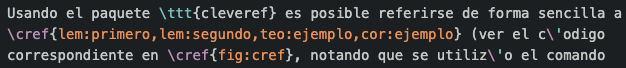
\includegraphics[width=0.8\textwidth]{recursos/capturas/cref}
  \caption{Ejemplo de uso de \ttt{\textbackslash{cref}}.}
  \label{fig:cref}
\end{figure}

Sin embargo, la gram\'atica del espa\~nol hace necesario introducir variantes en
algunos casos especiales, como cuando hacemos referencia ``al Teorema
\ref{teo:ejemplo}'' (n\'otese que se utiliz\'o ``al Teorema'' en lugar de ``el
Teorema''), o queremos decir que un resultado es una consecuencia ``del
Corolario \ref{cor:ejemplo}''.   En este caso, necesitamos agregar el nombre del
ambiente a mano, y usar el comando habitual \ttt{\textbackslash{ref}}.   El
autor del presente documento prefiere utilizar siempre may\'usculas cuando se
usa el nombre de un ambiente referido por n\'umero, e.g., ``\cref{teo:ejemplo}''
en lugar de ``el teorema \ref{teo:ejemplo}'', por lo que esta configuraci\'on se
ve reflejada en el archivo \ttt{tesis.tex}, cuando se utiliza el comando
\ttt{\textbackslash{crefname}} para definir los nombres de ambiente que debe de
usar \ttt{cleveref}.

Una alternativa para evitar algunos de los problemas descritos en el p\'arrafo
anterior es definir el nombre del ambiente sin utilizar el art\'iculo, e.g.,
``Teorema'' en lugar de ``el Teorema''.   Aunque esto permite un poco m\'as de
flexibilidad, cuando es necesario cambiar un ambiente con nombre masculino a uno
con nombre femenino, o viceversa (por ejemplo proposici\'on por lema), es
necesario realizar todos los cambios de los art\'iculos a mano.  Adicionalmente,
(y el motivo principal por el que se decidi\'o no usar esta variante) el uso del
paquete como el mostrado en el ejemplo de \cref{fig:cref} dejar\'ia de
funcionar, pues los art\'iculos ser\'ian omitidos, generando una construcci\'on
gramatical incorrecta.

Si no se desea usar el paquete \ttt{cleveref}, siempre puede omitirse y utilizar
\'unicamente el comando \ttt{\textbackslash{ref}} que est\'a incluido por
omisi\'on en \LaTeX.

Adem\'as de los ambientes, tambi\'en es posible etiquetar cap\'itulos o
secciones, y referirnos a la p\'agina donde aparece una etiqueta dada.   Por
ejemplo, podemos referirnos a \cref{sec:dibujos} en la \cpageref{sec:dibujos}, o
al Cap\'itulo \ref{cap:ejemplos}.   La referencia a las p\'aginas es \'util en
la versi\'on impresa del documento, aunque en la versi\'on digital parezca un
poco in\'util gracias a que cada referencia es una liga al objeto en cuesti\'on.



\section{Dibujos y colores}
\label{sec:dibujos}

Los dibujos pueden agregarse de al menos dos formas obvias.   La primera es
hacerlos dentro de \LaTeX con alg\'un paquete como
\href{https://github.com/pgf-tikz/pgf}{\ttt{tikz}}\index{tikz}.   La segunda es
generarlos con alg\'un recurso externo, e incluirlo con el comando
\ttt{\textbackslash{includegraphics}}.   Tambi\'en puede usarse una
combinaci\'on de ambos, generando un PDF con la imagen en un archivo externo de
\LaTeX, y agreg\'andolo con \ttt{\textbackslash{includegraphics}}; una ventaja
de esta tercera posibilidad es que el compilador realiza menos trabajo para
generar el documento.

En \cref{fig:grafica} podemos ver un ejemplo de un dibujo hecho con \ttt{tikz}.
Una ventaja de hacer los dibujos dentro de \LaTeX{} es que resulta f\'acil
agregar f\'ormulas o etiquetas con la misma tipograf\'ia que el resto del
documento.

\begin{figure}[ht!]
\centering
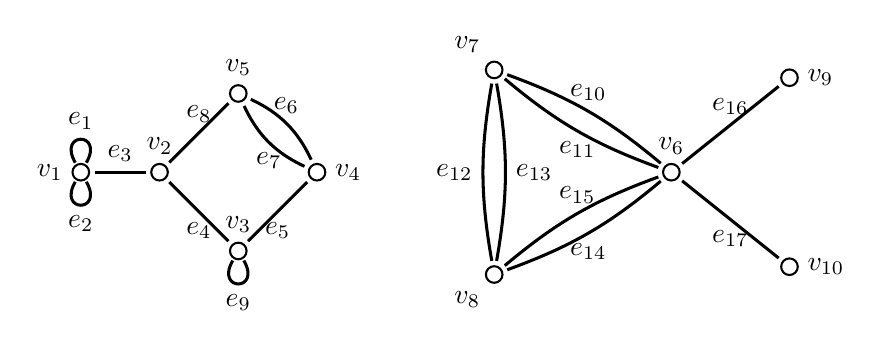
\begin{tikzpicture}
\node (0) [vertex,label=180:$v_1$] at (0,0){};
\node (1) [vertex,label=90:$v_2$]  at (1,0){};
\begin{scope}[xshift=2cm]
\node (2) [vertex,label=90:$v_3$]  at (270:1){};
\node (3) [vertex,label=0:$v_4$]   at (0:1){};
\node (4) [vertex,label=90:$v_5$]  at (90:1){};
\end{scope}

\draw [myloop,in=60,out=120,looseness=12]
      (0) to node[above]{$e_1$} (0);
\draw [myloop,in=240,out=300,looseness=12]
      (0) to node[below]{$e_2$} (0);
\draw [myloop,in=240,out=300,looseness=12]
      (2) to node[below]{$e_9$} (2);

\draw [edge]               (0) to node [above] {$e_3$} (1);
\draw [edge]               (1) to node [below] {$e_4$} (2);
\draw [edge]               (2) to node [below] {$e_5$} (3);
\draw [edge,bend right=20] (3) to node [above] {$e_6$} (4);
\draw [edge,bend left=20]  (3) to node [below] {$e_7$} (4);
\draw [edge]               (4) to node [above] {$e_8$} (1);


% Componente derecha
\begin{scope}[xshift=6cm]
\node (5) [vertex,label=90:$v_6$]    at (0:1.5){};
\node (6) [vertex,label=120:$v_7$]   at (120:1.5){};
\node (7) [vertex,label=240:$v_8$]   at (240:1.5){};
\node (8) [vertex,label=0:$v_9$]     at (3,1.2){};
\node (9) [vertex,label=0:$v_{10}$]  at (3,-1.2){};

\draw [edge,bend right=10] (5) to node [above] {$e_{10}$} (6);
\draw [edge,bend left=10]  (5) to node [below] {$e_{11}$} (6);
\draw [edge,bend right=10] (6) to node [left]  {$e_{12}$} (7);
\draw [edge,bend left=10]  (6) to node [right] {$e_{13}$} (7);
\draw [edge,bend right=10] (7) to node [below] {$e_{14}$} (5);
\draw [edge,bend left=10]  (7) to node [above] {$e_{15}$} (5);
\draw [edge]               (5) to node [above] {$e_{16}$} (8);
\draw [edge]               (5) to node [below] {$e_{17}$} (9);
\end{scope}

\end{tikzpicture}
\caption{El diagrama de una gr\'afica con lazos y
aristas m\'ultiples.}
\label{fig:grafica}
\end{figure}

Es f\'acil agregar colores a los dibujos.   Hay que tener presente que
\ttt{tikz} construye el dibujo por capas, y el c\'odigo se ejecuta de forma
secuencial, por lo que la \'ultima parte del c\'odigo es la \'ultima capa que se
dibujar\'a, y puede cubrir a otras, generando un resultado distinto al deseado.
Es posible definir colores nuevos mediante el comando
\ttt{\textbackslash{definecolor}}, en el caso de este documento, todos los
colores nuevos se definen en el archivo \ttt{tesis.tex}.   Las diferentes
opciones para el comando \ttt{\textbackslash{definecolor}} se encuentran
explicadas \href{https://en.wikibooks.org/wiki/LaTeX/Colors}{aqu\'i}.

Para agregar colores en el texto, o en las celdas de una tabla, u otros lugares,
se puede utilizar el paquete
\href{https://ctan.org/pkg/xcolor}{\ttt{xcolor}}\index{xcolor}.  Una forma
sencilla de usar color en el texto es con la construcci\'on
\begin{lstlisting}
{\color{nombre-del-color}texto con color}}
\end{lstlisting}
{\color{verdeAzulado}lo que permite generar texto de color.

Incluso es posible usar un color a lo largo de distintos p\'arrafos.}


\begin{figure}[ht!]
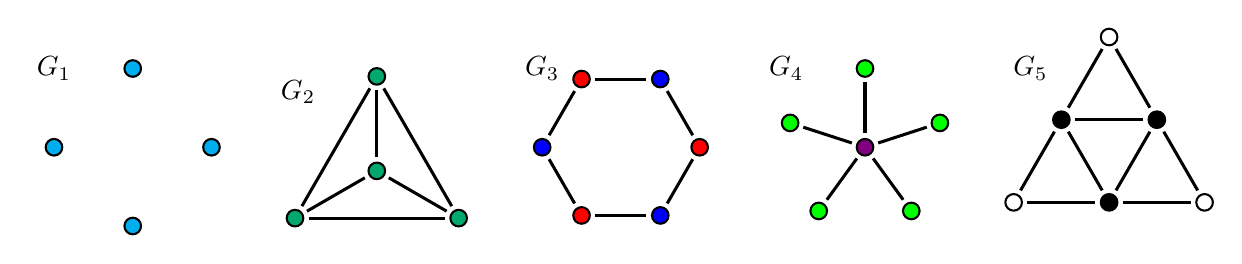
\begin{tikzpicture}
%%%%%%%%%%%%%%%%%%%%%%%%%%%%%%%%%%%%%%%%%%%%%%%%
%%%%%%%%%%         Empty Graph        %%%%%%%%%%
%%%%%%%%%%%%%%%%%%%%%%%%%%%%%%%%%%%%%%%%%%%%%%%%
\begin{scope}
% if label is needed -> label={(360/4)*\i}:$\i$
\foreach \i in {0,...,3}
	\node (\i) [vertex,fill=cyan] at ({(360/4)*\i}:1){};

\node (L) at (-1,1){$G_1$};
\end{scope}

%%%%%%%%%%%%%%%%%%%%%%%%%%%%%%%%%%%%%%%%%%%%%%%%
%%%%%%%%%%       Complete Graph       %%%%%%%%%%
%%%%%%%%%%%%%%%%%%%%%%%%%%%%%%%%%%%%%%%%%%%%%%%%
\begin{scope}[xshift=3.1cm,yshift=-0.3cm]
\node (4) [vertex,fill=verdeAzulado] at (0,0){};
\foreach \i in {0,1,2}
	\node (\i) [vertex,fill=verdeAzulado] at ({90+(360/3)*\i}:1.2){};

\foreach \i in {0,1,2}
	\draw [edge] let \n1={int(mod(\i+1,3))} in (\i) to (\n1);
\foreach \i in {0,1,2}
	\draw [edge] (\i) to (4);

\node (L) at (-1,1){$G_2$};
\end{scope}


%%%%%%%%%%%%%%%%%%%%%%%%%%%%%%%%%%%%%%%%%%%%%%%%
%%%%%%%%%%       Bipartite Graph      %%%%%%%%%%
%%%%%%%%%%%%%%%%%%%%%%%%%%%%%%%%%%%%%%%%%%%%%%%%
\begin{scope}[xshift=6.2cm,yshift=0cm]
\foreach \i in {0,2,4}
	\node (\i) [vertex,fill=red]  at ({(360/6)*\i}:1){};
\foreach \i in {1,3,5}
	\node (\i) [vertex,fill=blue] at ({(360/6)*\i}:1){};

\foreach \i in {0,...,5}
	\draw [edge] let \n1={int(mod(\i+1,6))} in (\i) to (\n1);

\node (L) at (-1,1){$G_3$};
\end{scope}


%%%%%%%%%%%%%%%%%%%%%%%%%%%%%%%%%%%%%%%%%%%%%%%%
%%%%%%%%%%            Star            %%%%%%%%%%
%%%%%%%%%%%%%%%%%%%%%%%%%%%%%%%%%%%%%%%%%%%%%%%%
\begin{scope}[xshift=9.3cm]
\node (6) [vertex,fill=violet] at (0,0){};
\foreach \i in {0,...,4}
	\node (\i) [vertex,fill=green] at ({90+(360/5)*\i}:1){};

\foreach \i in {0,...,4}
	\draw [edge] (\i) to (6);

\node (L) at (-1,1){$G_4$};
\end{scope}


%%%%%%%%%%%%%%%%%%%%%%%%%%%%%%%%%%%%%%%%%%%%%%%%
%%%%%%%%%%           Split            %%%%%%%%%%
%%%%%%%%%%%%%%%%%%%%%%%%%%%%%%%%%%%%%%%%%%%%%%%%
\begin{scope}[xshift=12.4cm]
\foreach \i in {0,2,4}
	\node (\i) [vertex,fill=black] at ({30+(360/6)*\i}:0.7){};
\foreach \i in {1,3,5}
	\node (\i) [vertex] at ({30+(360/6)*\i}:1.4){};

\foreach \i in {0,...,5}
	\draw [edge] let \n1={int(mod(\i+1,6))} in (\i) to (\n1);
\foreach \i in {0,2,4}
	\draw [edge] let \n1={int(mod(\i+2,6))} in (\i) to (\n1);

\node (L) at (-1,1){$G_5$};
\end{scope}

\end{tikzpicture}
\caption{Ejemplos de gr\'aficas vac\'ia, completa,
bipartita, bipartita completa y escindible.}
\label{fig:fam1}
\end{figure}

Continuando con los dibujos, resulta bastante \'util usar ciclos \ttt{for}
dentro de \ttt{tikz} para realizar dibujos que tienen simetr\'ias.   Un ejemplo
de esto ocurre en \cref{fig:fam1}.   En \cref{fig:tikzFor}, se observa el
c\'odigo del ciclo azul y rojo que aparece en \cref{fig:fam1}.

\begin{figure}[ht!]
  \centering
  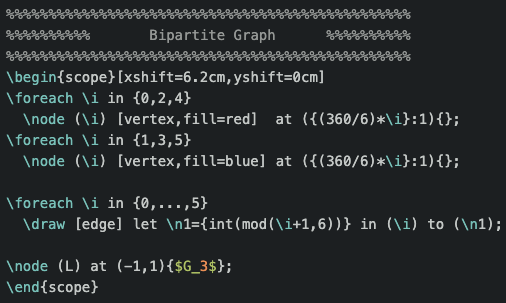
\includegraphics[width=0.8\textwidth]{recursos/capturas/tikzfor}
  \caption{Ejemplo de un ciclo \ttt{for} dentro de \ttt{tikz}.}
  \label{fig:tikzFor}
\end{figure}

Aunque en este caso los ejemplos se concentran en dibujar gr\'aficas, las
posibilidades de \ttt{tikz} son gigantescas.   Se recomienda al usuario revisar
el \href{https://mirror.las.iastate.edu/tex-archive/graphics/pgf/base/doc/%
pgfmanual.pdf}{manual de PGF y TikZ}.


\section{Algoritmos}

Para los algoritmos utilizamos el paquete \href{https://www.ctan.org/pkg/%
algorithm2e}{\ttt{algorithm2e}}\index{algorithm2e}.   En este caso simplemente
se presentar\'a un ejemplo de uso con un subconjunto limitado de las distintas
opciones que se pueden utilizar.   Se recomienda revisar la documentaci\'on del
paquete para conocer todas las posibilidades.

\begin{algorithm}[ht!]
\SetAlgorithmName{Algoritmo}{}
  \DontPrintSemicolon
  \SetKwData{False}{false}\SetKwData{True}{true}
  \SetKwFunction{New}{new}\SetKwFunction{End}{end}\SetKwFunction{Used}{used}
  \SetKwInOut{Input}{input}\SetKwInOut{Output}{output}

  \KwIn{Una gr\'afica conexa $G$ con un v\'ertice distingido $r$.}
  \KwOut{Funciones de parentesco $p$, nivel $\ell$ y tiempo de exploraci\'on
         $t$.}
  \BlankLine
  $Q \leftarrow []$; $i \leftarrow 0$\;
  $i \leftarrow i+1$\;
  colorear a $r$ de negro\;
  a\~nadir $r$ al final de $Q$\;
  $t(r) \leftarrow i$, $p(r) \leftarrow \varnothing$, $\ell (r) \leftarrow 0$\;
  {\While{$Q \ne []$}{
  	elegir a la cabeza $x$ de $Q$\;
 	\If{$x$ tiene un vecino $y$ sin colorear}{
		$i \leftarrow i+1$\;
		colorear a $y$ de negro\;
		a\~nadir $y$ al final de $Q$\;
		$t(y) \leftarrow i$, $p(y) \leftarrow x$, $\ell(y) \leftarrow \ell(x) + 1$\;
	}\Else{
		eliminar $x$ de $Q$\;
	}
  }
  }
  {\Return $(p,\ell,t)$}
  \caption{Breadth First Search}
  \label{alg:bfs}
\DecMargin{1em}
\end{algorithm}

\Cref{alg:bfs} muestra algunas opciones sencillas del paquete.   Quiz\'a la
observaci\'on m\'as importante para considerar respecto a \ttt{algorithm2e} es
que, por dise\~no, el paquete no divide los algoritmos para aparecer en m\'as
de una p\'agina.   Por lo tanto, un algoritmo largo usualmente se recorrer\'a
a la siguiente p\'agina (y posiblemente ocupar\'a una p\'agina completa).

\section{\'Indice alfab\'etico}
\label{sec:indice}

Es posible agregar palabras al \'indice\index{indice@\'indice} alfab\'etico
usando el comando \ttt{\textbackslash{index}}.   Un uso t\'ipico es el
siguiente; supongamos que se desea agregar la palabra ``gr\'afica'' al \'indice,
entonces es necesario escribir la palabra, seguida de la misma palabra dentro
del comando.
\begin{lstlisting}
gr\'afica\index{gr\'afica}
\end{lstlisting}

Cuando se introduce un concepto nuevo, es deseable resaltarlo de alguna forma en
el texto.   En los art\'iculos usualmente se utilizan \textit{cursivas} y en los
libros (o una tesis), generalmente se prefieren las \textbf{negritas}.   Por
este motivo, se agreg\'o al pre\'ambulo un comando para poner, al mismo tiempo,
una palabra en negritas y agregarla al \'indice; el comando es
\ttt{\textbackslash{indice}}.   Por ejemplo, dicho comando est\'a siendo
utilizado en la palabra \indice{concepto}, mismo que se puede verificar aparece
en el \'indice anal\'itico al final del documento. Tambi\'en es com\'un
encontrar una versi\'on especializada de un concepto, e.g., la definici\'on de
gr\'afica bipartita depende de la de gr\'afica.   En este sentido, es deseable
que ``gr\'afica bipartita'' aparezca como una entrada que depende de
``gr\'afica''.   Para lograr esto se utiliza el mismo comando
\ttt{\textbackslash{index}}, con la siguiente sintaxis.
\begin{lstlisting}
\index{concepto!subconcepto}
\end{lstlisting}

De manera an\'aloga al caso del comando \ttt{\textbackslash{indice}}, se cre\'o
un comando \ttt{\textbackslash{indiceSub}}, que toma dos argumentos.  El primero
es la entrada principal que aparecer\'a en el \'indice (e.g., gr\'afica), y la
segunda es la versi\'on especializada que depende de la primera (e.g.,
bipartita).   Para brindar libertad en la forma de redactar las definiciones,
\ttt{\textbackslash{indiceSub}} s\'olo imprime en el documento el segundo
argumento.   Por ejemplo, en \indiceSub{concepto}{subconcepto} se utiliz\'o
\ttt{\textbackslash{indiceSub}} con los argumentos \ttt{concepto} y
\ttt{subconcepto} (puede verificarse el funcionamiento en el \'indice).

Dependiendo del editor que se est\'e utilizando para trabajar con \LaTeX, es
posible que el \'indice no se actualice autom\'aticamente.   De ser el caso,
basta con ejecutar el siguiente comando en el directorio del proyecto donde se
encuentre el archivo \ttt{tesis.idx} (\'este \'ultimo se genera
autom\'aticamente al compilar \ttt{tesis.tex}).
\lstset{language=bash}
\begin{lstlisting}
makeindex tesis.idx
\end{lstlisting}

El comando anterior generar\'a el archivo \ttt{tesis.ind}, mismo que contiene la
informaci\'on necesaria para incluir el \'indice en el PDF final.

Los conceptos aparecen en orden alfab\'etico en el \'indice, sin embargo, el uso
de caracteres especiales (como letras acentuadas) afecta el orden habitual.
Para corregir problemas derivados del uso de caracteres especiales, se refiere
al lector al siguiente \href{https://en.wikibooks.org/wiki/LaTeX/%
Indexing#Using_special_characters}{art\'iculo sobre indexaci\'on}.

\chapter{Polic\'ias y ladrones sobre gr\'aficas de fichas de \'arboles}
\label{cap:resultados}

\section{Estrellas}

\begin{lema}
\label{lem:isomorfismo}
    Sean $k$ y $n$ enteros positivos. Si $G$ una gr\'afica de orden $n$ y $k <
    n$, entonces $\t{k}{G} \cong \t{n-k}{G}$
\end{lema}

En virtud d\cref{lem:isomorfismo}, dado que $S_n$ tiene orden $n+1$ para cada
$n$ entero positivo, entonces para cada $k$ en los enteros positivos basta
analizar las gr\'aficas $S_n$ con $n\geq 2k-1$, pues si $n<2k-1$, v\'ease que
\[
    2\c{\paren{n+1}-k}-1 = 2n - (2k-1),
\]
y como $n<2k-1$, entonces
\[
    2\c{\paren{n+1}-k}-1 < 2n - n = n,
\]
por lo que en este caso, si $r=\paren{n+1}-k$, se tiene que $n\geq 2r-1$, de
manera que basta determinar $c\paren{\t{r}{S_n}}$ pues
$\t{k}{S_n}\cong\t{\paren{n+1}-k}{S_n} = \t{r}{S_n}$.

\begin{lema}
\label{lem:desigualdad}
    Para cualquier $k\geq 2$, $\ds\binom{2k-1}{k-1} > k\paren{k-1}$.
\end{lema}

\begin{proof}
    Desarrollando de la formula del binomio,
    \begin{align*}
           \binom{2k-1}{k-1} - k\paren{k-1}
        &= \frac{\paren{2k-1}!}{\paren{k-1}!\paren{2k-1-\paren{k-1}}!} -
           k\paren{k-1} \\
        &= \frac{\paren{2k-1}!}{\paren{k-1}!\paren{k}!} - k\paren{k-1} \\
        &= \frac{\paren{2k-1}\cdots \paren{k+1}}{\paren{k-1}!} - \frac{k
           \paren{k-1}\paren{k-1}!}{\paren{k-1}!} \\
        &= \frac{\paren{2k-1}\cdots \paren{k+1} - k\paren{k-1}
           \paren{k-1}!}{\paren{k-1}!}.
    \end{align*}

    Por tanto, es suficiente demostrar que el numerador de la \'ultima igualdad
    es mayor que cero. As\'i pues, v\'ease que
    \[
        k\paren{k-1}\paren{k-1}! = \paren{2k-2}\cdot \underbrace{\paren{k \cdot
        \paren{k-1}\cdots 4 \cdot 3}}_{k-2 \text{ t\'erminos}}.
    \]
    Luego, como $k\geq 2$ se tiene que $k+r \geq 2+r$ para cualquier $r\in\n$,
    de manera que los \'ultimos $k-2$ t\'erminos de la expresi\'on 
    \[
        \paren{2k-1}\cdots \paren{k+1}
    \]
    son mayores o iguales a los \'ultimos $k-2$ t\'erminos de
    $k\paren{k-1}\paren{k-1}!$. M\'as a\'un, $2k-1 > 2k-2$, de modo que
    \[
        \paren{2k-1}\cdots \paren{k+1} > k\paren{k-1}\paren{k-1},
    \]
    concluyendo as\'i que
    \[
        \binom{2k-1}{k-1} - k\paren{k-1} > 0.
    \]
\end{proof}

\begin{teorema}
\label{teo:cota_estrella}
    Para $k\geq 2$ y $n\geq 2k-1$, $c\paren{\t{k}{S_n}} \geq k$.
\end{teorema}

% Definiciones necesarias: estrategia de escape, configuración inicial,
% configuración dominada en su totalidad por un policía (es un subconjunto de
% v\'ertices de la configuraci\'on que ocupa). Notar que c_1,...c_k,
% representaran a los policías y c_i(j) representa la j-ésima ficha de c_i
% r_(1),..., r_(k) son las fichas del ladrón, r representa al ladrón.

\begin{proof}
    Basta demostrar que el ladr\'on tiene una estrategia de escape jugando sobre
    $\t{k}{S_{2k-1}}$ contra $k-1$ polic\'ias, notando que para $n > 2k-1$, el
    ladr\'on realiza los mismos movimientos, ignorando las hojas adicionales.

    Primero se demuestra que dada cualquier configuraci\'on inicial de fichas de
    los $k-1$ polic\'ias, el ladr\'on siempre puede escoger v\'ertices para
    posicionar sus fichas de manera que ning\'un polic\'ia le captura $k-1$
    fichas en las hojas. En efecto, n\'otese que el n\'umero de
    $\paren{k-1}$-conjuntos formados \'unicamente por hojas de $S_{2k-1}$ es
    $\binom{2k-1}{k-1}$. Por otra parte, si un polic\'ia coloca sus $k$ fichas
    sobre las hojas, este domina $\binom{k}{k-1}$ de estos
    $\paren{k-1}$-conjuntos. En este orden de ideas, los $k-1$ polic\'ias pueden
    dominar en su totalidad $k\paren{k-1}$ de los $\paren{k-1}$-conjuntos
    formados por hojas, de manera que, por \cref{lem:desigualdad}, el ladr\'on
    siempre puede escoger una configuraci\'on de $k-1$ hojas que no est\'e
    dominada en su totalidad por un polic\'ia, escogiendo el v\'ertice $0$ para
    posicionar su \'ultima ficha y sobreviviendo su primer turno. 

    \begin{figure}[h]
        \centering
        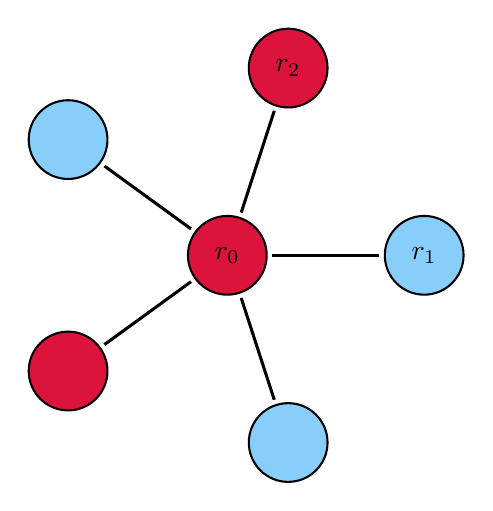
\begin{tikzpicture}[every node/.style = {draw, circle, minimum size=1cm,
            line width=0.75pt, inner sep=0pt, outer sep=0pt}] \node (0)
            [fill=Crimson] at (0,0) {$r_0$}; \node (1) [fill=LightSkyBlue] at
            ({360/5 * (1 - 1)}:2.5cm) {$r_1$}; \node (2) [fill=Crimson] at
            ({360/5 * (2 - 1)}:2.5cm) {$r_2$}; \node (4) [fill=Crimson] at
            ({360/5 * (4 - 1)}:2.5cm) {}; \foreach \s in {3,5}{ \node (\s)
            [fill=LightSkyBlue] at ({360/5 * (\s - 1)}:2.5cm) {}; } \foreach \s
            in {1,...,5} { \draw [edge] (\s) to (0); }
        \end{tikzpicture}
        \caption{Una posible elecci\'on de configuraci\'on inicial de $R$ para
        $k=3$. N\'otese que ninguno de los $k-1$ polic\'ias, cuyas posiciones de
        fichas est\'an representadas por los colores azul y rojo, est\'an
        capturando dos fichas de $R$ en las hojas.}
        \label{fig:Configuracion_inicial}
    \end{figure}

    Sean $c_1,\dots, c_{k-1}$ los polic\'ias. Determinada la disposici\'on
    inicial de las fichas, n\'otese que el ladr\'on no puede ser capturado en el
    siguiente movimiento de los polic\'ias pues, dada la elecci\'on de
    configuraci\'on, si existe $i\in\seg{1}{k-1}$ tal que $c_i$ est\'a
    capturando a $k-1$ de las fichas de $R$, entonces necesariamente una de las
    fichas de $c_i$ est\'a en el centro, de manera que necesita al menos $2$
    movimientos para capturar todas las fichas de $r$ (uno para capturar la hoja
    que le falta y uno para recapturar la ficha del centro). Por tanto, el
    ladr\'on sobrevive al turno de los polic\'ias y revisa si despu\'es de sus
    movimientos este ha quedado con $k-1$ fichas en las hojas capturadas por un
    mismo polic\'ia. De no ser as\'i, el ladr\'on asegura su supervivencia hasta
    su siguiente turno al igual que posterior a la elecci\'on de configuraci\'on
    inicial, por lo que se limita a pasar. De lo contrario, este debe mover su
    ficha en $0$.
    
    N\'otese que en un mismo turno varios polic\'ias pudieron haber completado
    sus $k-1$ capturas en las hojas donde se encuentran las fichas del ladr\'on.
    Sea $m$ un entero positivo y sup\'ongase sin p\'erdida de generalidad que
    $c_{1},\dots, c_{m}$ son los polic\'ias que han capturado las $k-1$ fichas
    de $r$ en las hojas. Dado que cada $c_{i}$ pas\'o de no estar capturando a
    capturar las $k-1$ fichas de $R$ en hojas, entonces necesariamente en esta
    nueva instancia dichos polic\'ias no tienen una ficha en $0$ (pues una de
    sus fichas se movi\'o de ah\'i para capturar la hoja que les faltaba,
    respectivamente). As\'i, por cada uno de estos polic\'ias, $R$ tiene una
    hoja menos a la cual puede mover su ficha en $0$, pues perder\'ia el juego
    inmediatamente. De este modo, en el peor de los casos, hay $m+k-1$ hojas no
    disponibles de las $2k-1$, donde las $k-1$ corresponden a las hojas en las
    que $R$ ya tiene una ficha.

    Luego, el resto de hojas disponibles pueden estar ocupadas por alguna ficha
    de  $c_{{m+1}},\dots,c_{{k-1}}$, quienes al final de su turno no estaban
    capturando las $k-1$ fichas en hojas de $R$. Si alguno de estos polic\'ias
    tiene una de sus fichas en $0$ y est\'a capturando $k-2$ de las $k-1$ fichas
    en hojas de $R$, entonces el ladr\'on tiene una hoja menos a la cual puede
    moverse, pues de hacerlo, este provocar\'ia que tal polic\'ia le capture
    $k-1$ fichas en hojas y bastar\'ia con mover su ficha en $0$ a la hoja que
    le falta capturar. Nuevamente el peor de los casos implicar\'ia que hay
    otras $k-1-m$ hojas no disponibles para $R$ (una correspondiente a cada
    $c_i$ con $i>m$). As\'i, $R$ tiene a lo m\'as $m+k-1+k-1-m=2k-2$ hojas no
    disponibles de las $2k-1$, por lo que este siempre tendr\'a al menos una
    hoja a la cual se puede mover de manera que no incremente la cantidad de
    polic\'ias que se encuentran capturando $k-1$ fichas en sus hojas.

    En el siguiente turno, si ninguno de los $c_{i}$ con $i\in\seg{1}{m}$ mueve
    su \'ultima ficha que no est\'a capturando a $0$, entonces $R$ pasa.
    N\'otese que los polic\'ias $c_{m+1},\dots,c_{{k-1}}$ pueden seguir moviendo
    sus fichas y, eventualmente, pueden llegar a agregarse al conjunto de
    polic\'ias que est\'an capturando $k-1$ fichas en las hojas, por lo que en
    cada uno de los movimientos de los polic\'ias puede que $m$ aumente (o
    disminuya) y haya que realizar un reetiquetado de los polic\'ias para
    identificar qui\'enes de estos son los m\'as cercanos a capturar. M\'as
    a\'un, en caso de que $m$ aumente, cada polic\'ia que se encuentran
    capturando $k-1$ fichas de $R$ en las hojas no tiene una ficha en $0$, pues
    debi\'o haber usado esa para capturar, asegurando que $R$ puede sobrevivir
    un turno m\'as.

    En el peor caso, los polic\'ias $c_1,\dots, c_m$ mueven su ficha que no
    est\'a capturando a $0$. Se afirma entonces que $R$ tiene una ficha que
    est\'a siendo simult\'aneamente capturada por cada $c_{i}$ con $i\in
    \seg{1}{m}$. En efecto, al ser $k-1$ polic\'ias y al estar capturando $k-1$
    fichas de las $k$ del ladr\'on, en el peor caso se tiene que a cada
    polic\'ia le falta una ficha distinta por capturar, de manera que, sin
    p\'erdida de generalidad, a $c_{i}$ le falta capturar la ficha $r_i$.
    Finalmente, como $m\leq k-1$, entonces al menos cada $c_{i}$ siempre
    estar\'a capturando la ficha $r_k$, de manera que $R$ procede a mover a la
    ficha $r_k$ a $0$. De este modo, $R$ vuelve a la situaci\'on inicial en la
    que ning\'un polic\'ia le est\'e capturando $k-1$ fichas en las hojas, por
    lo que el ladr\'on puede iterar este algoritmo para nunca ser capturado por
    alg\'un polic\'ia. Se concluye entonces que $c\paren{\t{k}{S_{2k-1}}} \ge
    k$.   
\end{proof}

%definir instancia de un juego de policías y ladrones y como se obtiene
%legalmente una de otra, [c_k]=el conjunto de
%fichas de c, [r_k]=el conjunto de fichas de r. c_{i,j}(t) representa la
%posición (vertice) de la j-ésima ficha del i-ésimo policía en el turno t.
Dado este resultado, nuestra nueva meta es determinar con exactitud el n\'umero
policiaco para las gr\'aficas de fichas de las estrellas. En las demostraciones
que siguen se utilizar\'a recurrentemente la estrategia descrita a
continuaci\'on. Consid\'erese una instancia $I$ del juego de polic\'ias y
ladrones sobre la gr\'afica de $k$ fichas de un \'arbol $T$. Dado $c$ un
polic\'ia, sup\'ongase que existe una funci\'on objetivo, $o \colon \c{c_k}\to
\c{r_k}$, tal que $c_i\mapsto r_i$ para cada $i\in\seg{1}{k}$; llamamos a $r_i$
el \textit{objetivo} de $c_i$. Se dice que una ficha $c_i$ est\'a
\textbf{obstruida} si no se encuentra capturando a su objetivo en el turno $t$
(i.e., $c_i(t)\neq r_i(t)$) y existe $c_j$ tal que $c_j(t)$ es el segundo
v\'ertice de la \'unica $c_i(t)r_i(t)$-trayectoria en $T$. En este caso se dice
que $c_j$ es una obstrucci\'on para $c_i$ en la instancia $I(t)$ (ver
\cref{fig:obstruccion}). Si adem\'as $c_i$ es una obstrucci\'on para $c_j$, se
dice que $c_i$ y $c_j$ se obstruyen mutuamente.

\begin{figure}[h]
    \centering
    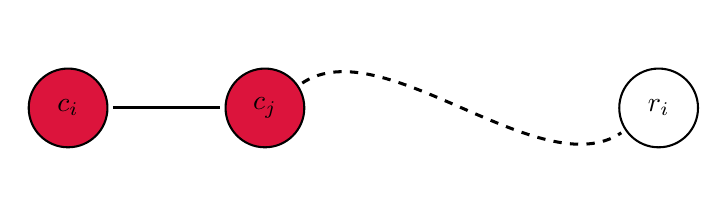
\begin{tikzpicture}[every node/.style = {draw, circle, minimum size=1cm,
        line width=0.75pt, inner sep=0pt, outer sep=0pt}, on grid, node distance
        = 2.5cm] \node (i) [fill=Crimson] {$c_i$}; \node (j) [fill=Crimson,
        right= of i] {$c_j$}; \node (1) [right=5cm of j] {$r_i$}; \draw[edge]
        (i) -- (j); \draw[dashed,edge] (j) .. controls (4,1) and (6,-1) .. (1);
    \end{tikzpicture}
    \caption{Diagrama de la ficha $c_i$ obstruida por la ficha $c_j$.}
    \label{fig:obstruccion}
\end{figure}

En caso de tener esta obstrucci\'on, n\'otese que $c$ es incapaz de acercar su
$i$-\'esima ficha a $r_i$ sin antes remover $c_j$ del v\'ertice $c_j(t)$. As\'i,
\cref{alg:desob} da una respuesta a c\'omo atender esta situaci\'on de manera
que la suma de las distancias de las fichas de $c$ a sus objetivos disminuye
(cuando el polic\'ia $c$ a\'un no se encuentra capturando a $R$).

%Mencionar que la suma de las distancias de las fichas a sus objetivos es mayor
%o igual a la distancia de c a R en la gráfica de fichas. El lema reduce la suma
%de distancias de fichas a sus objetivos, y la estrategia del teorema asegura
%que dicha suma se reduce en cada turno.

\begin{algorithm}[ht!]
    \SetAlgorithmName{Algoritmo}{}
      \DontPrintSemicolon
      \SetKwData{False}{false}\SetKwData{True}{true}
      \SetKwFunction{New}{new}\SetKwFunction{End}{end}\SetKwFunction{Used}{used}
      \SetKwInOut{Input}{input}\SetKwInOut{Output}{output}
    
      \KwIn{Un entero positivo $k$, un \'arbol $T$, una instancia $I(t)$ de un
      juego de un polic\'ias y ladrones con $k$ fichas sobre un \'arbol $T$ y
      $c_j$ una obstrucci\'on de $c_i$ en la instancia $I(t)$.} \KwOut{Una
      instancia $I(t+1)$ obtenida legalmente de $I(t)$ tal que la suma de las
      distancias de cada ficha de los polic\'ias a sus objetivos es
      estrictamente menor que en $I(t)$.}
      \BlankLine
      \If{$c_i$ y $c_j$ se obstruyen mutuamente}{
      define $I(t+1)$ como la instancia $I(t)$ con las etiquetas de $c_i$ y $c_j$ intercambiadas\;
      }\Else{
            \If{$c_j(t)=r_i(t)$ \label{line:c-sobre-r}}{
                \If{$c_j$ est\'a obstruido por alg\'un $c_s$}{
                    define $I(t+1) = \textsc{Desobstrucci\'on}
                    (k,T,I(t),c_s,c_j)$\;
                }\Else{
                    define $I(t+1)$ como la instancia $I(t)$ con la ficha $c_j$
                    en el segundo v\'ertice de la $c_j(t)r_j(t)$-trayectoria\;
                }
            }\Else{
                redefine $I(t)$ como la instancia $I(t)$ con las etiquetas de
                $c_i$ y $c_j$ intercambiadas\;
                \If{$c_i$ est\'a obstruido por alg\'un $c_s$}{
                    define $I(t+1) = \textsc{Desobstrucci\'on}
                    (k,T,I(t),c_s,c_i)$\; \label{line:llamada2}
                }\Else{
                    define $I(t+1)$ como la instancia $I(t)$ con la ficha $c_i$
                    en el segundo v\'ertice de la $c_i(t)r_i(t)$-trayectoria\;
                    \label{line:movimiento2}
                }
            }
        }
      {\Return $I(t+1)$}
      \caption{\textsc{Desobstrucci\'on}}
      \label{alg:desob}
    \DecMargin{1em}
    \end{algorithm}

En este orden de ideas, el siguiente lema demuestra la validez
d\cref{alg:desob}.

\begin{lema}
\label{lem:obstruccion}
    El Algoritmo \ref{alg:desob} es correcto.
\end{lema}

\begin{proof}
    Se identifican los siguientes casos dependiendo del tipo de obstrucci\'on:
    \begin{enumerate}
        \item Si $c_i$ y $c_j$ se obstruyen mutuamente (ver
        \cref{fig:obsmutua}), n\'otese que basta que se intercambien las
        etiquetas de estas fichas pues esto propicia que la distancia de ambas
        fichas a sus respectivos objetivos se reduzca en $1$ y $c_i$ y $c_j$
        dejan de obstruirse una a la otra. 
    
        \begin{figure}[ht!]
            \begin{tcbitemize}[raster columns=2,raster equal height, enhanced,
                colback=Black!5!white,colframe=Grey!75!black, raster every
                box/.style={minimum for current equal height group=2.5cm,
                valign=center, halign=center}, boxsep=0mm]
                \tcbitem 
                \begin{tikzpicture}
                    \node (i) [bola,fill=Crimson] {$c_i$};
                    \node (j) [bola,fill=Crimson, right=0.5cm of i] {$c_j$};
                    \node (1) [bola,right=1cm of j] {$r_i$};
                    \node (2) [bola,left=1cm of i] {$r_j$};
                    \draw[edge] (i) -- (j);
                    \draw[dashed,edge] (j) .. controls (2.25,1) and (2.75,-1) ..
                    (1);
                    \draw[dashed,edge] (i) .. controls (-0.75,1) and (-1.25,-1)
                    .. (2);
                \end{tikzpicture}
                \tcbitem
                \begin{tikzpicture}[every node/.style = {draw, circle, minimum
                    size=1cm, line width=0.75pt, inner sep=0pt, outer sep=0pt}]
                    \node (i) [bola,fill=Crimson] {$c_j$};
                    \node (j) [bola,fill=Crimson, right=0.5cm of i] {$c_i$};
                    \node (1) [bola,right=1cm of j] {$r_i$};
                    \node (2) [bola,left=1cm of i] {$r_j$};
                    \draw[edge] (i) -- (j);
                    \draw[dashed,edge] (j) .. controls (2.25,1) and (2.75,-1) ..
                    (1);
                    \draw[dashed,edge] (i) .. controls (-0.75,1) and (-1.25,-1)
                    .. (2);
                \end{tikzpicture}
            \end{tcbitemize}
            \caption{Si $c_i$ y $c_j$ se obstruyen mutuamente, entonces las
            fichas de $c$ reciben un reetiquetado, de manera que todas conservan
            sus objetivos salvo $c_i$ y $c_j$, que los intercambian.}
            \label{fig:obsmutua}
        \end{figure}

        \item Si $c_i$ y $c_j$ no se obstruyen mutuamente, se generan dos
            subcasos:
        \begin{enumerate}
            \item Si $r_i(t)=c_j(t)$, entonces $c_j$ a\'un no se se encuentra
            capturando su respectivo $r_j$ y la $c_j(t)r_j(t)$-trayectoria, $P$,
            no contiene a $c_i(t)$, de manera que $c$ puede mover su $j$-\'esima
            ficha al segundo v\'ertice de $P$. Si $c_j$ no se encuentra
            obstruida, entonces avanza a dicho v\'ertice, reduciendo la
            distancia a su objetivo y dejando libre el paso para $c_i$ tal como
            se muestra en \cref{fig:obsad1}. De lo
            contrario, el algoritmo se llama a s\'i mismo para resolver la nueva
            obstrucci\'on entre $c_j$ y $c_s$ (ver \cref{fig:obsad2}).

            \begin{figure}[ht!]
                \begin{tcbitemize}[raster columns=2,raster equal height,
                    enhanced, colback=Black!5!white,colframe=Grey!75!black,
                    raster every box/.style={minimum for current equal height
                    group=2.5cm, valign=center, halign=center}, boxsep=0mm]
                    \tcbitem 
                    \begin{tikzpicture}
                        \node (i) [bola,fill=Crimson] {$c_i$};
                        \node (j) [bola,fill=Crimson,right=0.5cm of i] {$c_j,
                        r_i$};
                        \node (1) [bola,right=0.5cm of j] {};
                        \node (2) [bola,right=1.5cm of 1] {$r_j$};
                        \draw[edge] (i) -- (j);
                        \draw[edge] (j) -- (1);
                        \draw[dashed,edge] (1) .. controls (3.875,1) and
                        (4.625,-1) .. (2);
                    \end{tikzpicture}
                    \tcbitem
                    \begin{tikzpicture}
                        \node (i) [bola,fill=Crimson] {$c_i$};
                        \node (j) [bola,right=0.5cm of i] {$r_i$};
                        \node (1) [bola,fill=Crimson, right=0.5cm of j] {$c_j$};
                        \node (2) [bola,right=1.5cm of 1] {$r_j$};
                        \draw[edge] (i) -- (j);
                        \draw[edge] (j) -- (1);
                        \draw[dashed,edge] (1) .. controls (3.875,1) and
                        (4.625,-1) .. (2);
                    \end{tikzpicture}
                \end{tcbitemize}
                \caption{Al no haber obstrucci\'on mutua entre $c_i$ y $c_j$,
                $c_j$ debe avanzar (de ser posible) siguiendo la $c_j(t)r_j(t)
                $-trayectoria.}
                \label{fig:obsad1}
            \end{figure}

            \begin{figure}[ht!]
                \begin{tcbitemize}[raster columns=2,raster equal height,
                    enhanced, colback=Black!5!white,colframe=Grey!75!black,
                    raster every box/.style={minimum for current equal height
                    group=2.5cm, valign=center, halign=center}, boxsep=0mm]
                    \tcbitem 
                    \begin{tikzpicture}
                        \node (i) [bola,fill=Crimson] {$c_i$};
                        \node (j) [bola,fill=Crimson,right=0.5cm of i] {$c_j,
                        r_i$};
                        \node (s) [bola,fill=Crimson,right=0.5cm of j] {$c_s$};
                        \node (2) [bola,right=1.5cm of s] {$r_j$};
                        \draw[edge] (i) -- (j);
                        \draw[edge] (j) -- (s);
                        \draw[dashed,edge] (s) .. controls (3.875,1) and
                        (4.625,-1) .. (2);
                    \end{tikzpicture}
                    \tcbitem
                    \begin{tikzpicture}
                        \node (j) [bola,fill=Crimson] {$c_j$};
                        \node (s) [bola,fill=Crimson, right=0.5cm of j] {$c_s$};
                        \node (2) [bola,right=3cm of s] {$r_j$};
                        \draw[edge] (j) -- (s);
                        \draw[dashed,edge] (s) .. controls (2.75,1) and
                        (4.25,-1) .. (2);
                    \end{tikzpicture}
                \end{tcbitemize}
                \caption{Como $c_j$ est\'a obstruido, el algoritmo pasa a
                enfocarse a resolver la obstrucci\'on para $c_j$, $c_s$.}
                \label{fig:obsad2}
            \end{figure}

            \item Si $r_i(t)\neq c_j(t)$, $c_i$ y $c_j$ intercambian sus
            etiquetas, de modo que $c_j$ aumenta la distancia a su objetivo en
            $1$ y $c_i$ reduce la distancia a su objetivo en $1$ tal como se
            muestra en \cref{fig:obsnoad1}. Si $c_i$ no se
            encuentra obstruida, entonces esta ficha se mueve al segundo
            v\'ertice de la $c_j(t)r_i(t)$-trayectoria (que coincide con el
            tercer v\'ertice de la $c_i(t)r_i(t)$-trayectoria que se ten\'ia de
            la instancia $I(t)$), reduciendo la distancia a su objetivo otra
            unidad adicional. De lo contrario, el algoritmo se llama a s\'i
            mismo para resolver la nueva obstrucci\'on entre $c_i$ y $c_s$.

            \begin{figure}[ht!]
                \begin{tcbitemize}[raster columns=2,raster equal height,
                                   enhanced,
                                   colback=Black!5!white,colframe=Grey!75!black,
                                   raster every box/.style={minimum for current
                                   equal height group=2.5cm, valign=center,
                                   halign=center}, boxsep=0mm]
                    \tcbitem 
                    \begin{tikzpicture}
                        \node (i) [bola,fill=Crimson] {$c_i$};
                        \node (j) [bola,fill=Crimson, right=0.5cm of i] {$c_j$};
                        \node (1) [bola,right=1cm of j] {$r_i$};
                        \node (2) [bola,right=1cm of 1] {$r_j$};
                        \draw[edge] (i) -- (j);
                        \draw[dashed,edge] (j) .. controls (2.25,1) and
                        (2.75,-1) .. (1);
                        \draw[dashed,edge] (1) .. controls (4.25,1) and
                        (4.75,-1) .. (2);
                    \end{tikzpicture}
                    \tcbitem
                    \begin{tikzpicture}
                        \node (i) [bola,fill=Crimson] {$c_j$};
                        \node (j) [bola,fill=Crimson, right=0.5cm of i] {$c_i$};
                        \node (1) [bola,right=1cm of j] {$r_i$};
                        \node (2) [bola,right=1cm of 1] {$r_j$};
                        \draw[edge] (i) -- (j);
                        \draw[dashed,edge] (j) .. controls (2.25,1) and
                        (2.75,-1) .. (1);
                        \draw[dashed,edge] (1) .. controls (4.25,1) and
                        (4.75,-1) .. (2);
                    \end{tikzpicture}
                \end{tcbitemize}
                \caption{$c_i$ y $c_j$ intercambian sus etiquetas, de manera que
                $c_i$ se acerca en uno a su objetivo, pero $c_j$ se aleja en uno
                (not\'ando que lo mismo sucede si $r_j$ aparece antes de $r_i$
                en la trayectoria). De aqu\'i, el algoritmo decide qu\'e hacer
                con $c_i$ dependiendo de si esta se encuentra obstruida o no
                siguiendo la estrategia mostrada en \cref{fig:obsad1} o en
                \cref{fig:obsad2} (sustituyendo $c_j$ por $c_i$).}
                \label{fig:obsnoad1}
            \end{figure}
        \end{enumerate}
    \end{enumerate}

    V\'ease que el algoritmo tiene una ejecucci\'on finita pues las llamadas
        recursivas de la \cref{line:llamada2} generan nuevas instancias en las
        que $c_i$ recorre la $c_i(t)r_i(t)$-trayectoria inicial a trav\'es de
        reetiquetados de fichas, de manera que en cada uno de esos pasos la suma
        de las distancias de las fichas a sus respectivos objetivos se mantiene
        constante. Si en alguna de las llamadas recursivas sucede que $c_i$ deja
        de estar obstruida, entonces esta podr\'a ejecutar la instrucci\'on de
        la \cref{line:movimiento2}, reduciendo su distancia a $r_i$ en $1$ y,
        por tanto, reduciendo la suma de distancias de las fichas del polic\'ia
        a sus objetivos en $1$.
        
        De lo contrario, se tiene que $c_i$ llega a trav\'es de reetiquetados
        hasta estar a distancia $1$ de $r_i$, por lo que, o $c_i$ y $c_j$ se
        obstruyen mutuamente, en cuyo caso ya se vio que la suma de las
        distancias de las fichas de los polic\'ias a sus objetivos se reduce en
        $2$, o no se obstruyen mutuamente, de manera que en la siguiente llamada
        recursiva la ejecuci\'on entra al \texttt{if} de la
        \cref{line:c-sobre-r}.
        
        Al igual que en el caso anterior, si $c_j$ no est\'a obstruida, entonces
        esta puede avanzar al siguiente v\'ertice de la
        $c_j(t)r_j(t)$-trayectoria, reduciendo la distancia a su objetivo en $1$
        y, a su vez, reduciendo la suma de distancias de las fichas del
        polic\'ia a sus objetivos en $1$. Por otra parte, si $c_j$ est\'a
        obstruida, entonces esta ficha toma el lugar de $c_i$ en el algoritmo,
        de manera que la nueva meta es acercar a $c_j$ a su objetivo $r_j$, ya
        sea a trav\'es de reetiquetados o avanzando la ficha una posici\'on
        sobre la $c_j(t)r_j(t)$-trayectoria. Como en la \'ultima pasada
        recursiva no se entr\'o al \texttt{if} de la primera l\'inea, la
        $c_j(t)r_j(t)$-trayectoria no tiene a v\'ertice alguno de la
        $c_i(t)r_i(t)$-trayectoria salvo $c_j(t)=r_i(t)$, por lo que el
        algoritmo no vuelve a encontrarse con obstrucciones que ya ha
        reetiquetado. Esto implica que existe un momento en el que el algoritmo
        reetiqueta dos fichas que se obstruyen mutuamente o es capaz de mover
        una ficha del polic\'ia a un v\'ertice en el que no hab\'ia una ficha de
        \'el, concluyendo as\'i que el algoritmo finaliza y regresa una
        instancia en la que la suma de las distancias de las fichas del
        polic\'ia a sus respectivos objetivos se redujo.

\end{proof}

Con esta estrategia auxiliar estamos listos para determinar el n\'umero
policiaco para las gr\'aficas de $k$ fichas de las estrellas.

%Definir c_{i,j} es la j-esima ficha del i-esimo policia, perseguir.

\begin{teorema}
\label{teo:numero-de-policia-estrella}
    Para $k\geq 2$ y $n\geq 2k-1$, $c\paren{\t{k}{S_{n}}}=k$.
\end{teorema}

\begin{proof}
    Sean $c_1,\dots, c_k$ los $k$ polic\'ias. N\'otese que, al haber
    $\binom{k}{k-1}=k$ posibles $\paren{k-1}$-conjuntos de $\paren{c_1,\dots,
    c_k}$, es posible biyectar dichos $\paren{k-1}$-conjuntos con las $k$ fichas
    de $R$. M\'as a\'un, dado que cada polic\'ia tiene $k$ fichas, es posible
    que a cada uno de estos $\paren{k-1}$-conjuntos se les asignen, sin repetir,
    $k-1$ fichas, una por cada $c_i$ que aparezca en tal conjunto. En este
    sentido, a cada ficha de $R$, $r_i$, se le puede asociar un conjunto de
    $k-1$ fichas de polic\'ias distintos,
    $\overline{c_i}=\l{c_{1,i},\dots,c_{k,i}}\setminus\l{c_{i,i}}$. De este
    modo, como cada $c_i$ tiene una ficha en todos los $\overline{c_j}$ salvo
    para el $j=i$, entonces posterior a la asignaci\'on existe exactamente una
    ficha por cada polic\'ia a la que no se le asoci\'o ninguna ficha de $R$. En
    la estrategia descrita a continuaci\'on, cada polic\'ia $c_i$ ignora a $r_i$
    y se dedica a mover sus fichas para capturar a los $r_j$ con $j\neq i$,
    mientras que una de sus fichas, $c_{i,i}$, se le llamar\'a libre y no se
    mover\'a hasta que cada $\overline{c_j}$ est\'e capturando a $r_j$ (esto es,
    cada polic\'ia distinto de $c_j$ est\'a capturando a la ficha $r_j$ con sus
    $j$-\'esimas fichas). Obs\'ervese que esta asignaci\'on induce por cada
    polic\'ia una funci\'on objetivo dada por las etiquetas de las fichas de
    $c_i$ y $r_i$ (el objetivo de $c_{i,j}$ es $r_j$), la cual ser\'a utilizada
    cuando sea necesario resolver obstrucciones.

    Se afirma que es posible capturar cada $r_j$ con su correspondiente
    $\overline{c_j}$. Se ver\'a que en cada turno los polic\'ias son capaces de
    mantener el n\'umero de fichas del ladr\'on capturadas por un
    $\overline{c_i}$, y que despu\'es de un cierto n\'umero de turnos pueden
    aumentar la cantidad de fichas de $R$ capturadas por $\overline{c_i}$'s.

    Para la primera afirmaci\'on, si $R$ mueve $r_i$ tal que ya est\'a capturada
    por su correspondiente $\overline{c_i}$, entonces estas fichas proceden a
    perseguir al ladr\'on a donde sea que se mueva. Puede suceder que en la
    nueva posici\'on de $r_i$ se encuentren algunas de las fichas (posiblemente
    todas) de los polic\'ias que tienen una ficha en $\overline{c_i}$. En este
    caso, solo las fichas que no esten obstruidas se mueven a la nueva
    posici\'on de $r_i$, de manera que para el resto se ejecuta
    \cref{alg:desob}, por lo que para cada polic\'ia sucede que la suma de las
    distancias de sus fichas a sus objetivos se reduce y $\overline{c_i}$ vuelve
    a capturar a $r_i$.
    
    N\'otese adem\'as que recapturar con $\overline{c_i}$ y ejecutar
    \cref{alg:desob} representa un movimiento de a lo m\'as $k-1$ polic\'ias
    pues $c_i$ no tiene una ficha en $\overline{c_i}$, de manera que se puede
    acercar una ficha de $c_i$ en busca de completar otra captura con un
    $\overline{c_j}$ tal que $j\neq i$. V\'ease que esto siempre se puede hacer
    pues \cref{lem:obstruccion} implica que se pueden mover o reetiquetar fichas
    de $c_i$ para que la suma de las distancias a sus objetivos se reduzca.
    As\'i, si $c_i$ no puede mover ninguna de sus fichas hacia sus objetivos
    debido a obstrucciones, entonces es posible ejecutar \cref{alg:desob} para
    un par de fichas de $c_i$ que representen una obstrucci\'on, obteniendo como
    resultado una instancia en la que la suma de las distancias de sus fichas a
    sus objetivos se redujo \'unicamente con reetiquetados. Esto podr\'ia
    hacerse tantas veces como sea necesario hasta que la suma de las distancias
    sea igual a $0$ sin necesidad de hacer un solo movimiento de fichas de
    $c_i$, de manera que inicialmente $c_i$ ya estaba capturando a $R$ (pero sus
    fichas no capturaban a sus correspondientes objetivos).
    
    Por otra parte, para la segunda afirmaci\'on, consid\'erese que la
    configuraci\'on inicial de todos los polic\'ias es la misma y consiste en
    tener todas sus fichas en las hojas salvo una, que se encuentra en $0$, de
    manera que para cada $j\in \seg{1}{k}$, todas las fichas $c_{i,j}$ est\'an
    en un mismo v\'ertice y todas las fichas $c_{i,1}$ se encuentra en $0$.
    As\'i, en su primer turno los polic\'ias mueven para que $\overline{c_1}$
    capture a $r_1$ (suponiendo sin p\'erdida de generalidad que $r_1$ est\'a en
    una hoja), dejando que $c_{1,1}$ capture a alg\'un $r_j$ con $j\neq 1$.
    V\'ease que el ladr\'on no puede mover consecutivamente una infinidad de
    veces $r_1$ pues $C$ siempre podr\'ia recapturar y mover las fichas de $c_1$
    hacia sus respectivos objetivos, de manera que dicho polic\'ia capturar\'ia
    a $R$. As\'i, debe existir un primer momento en el que $R_1$ se queda fija
    (por al menos un turno). M\'as a\'un, si $R$ pasa en el resto de sus turnos,
    la misma estrategia puede usarse para que $c_1$ capture a $R$.

    Por tanto, como $R$ no puede pasar o mover $R_1$ indefinidamente, existe un
    turno en el cual $R$ realiza un movimiento con otra ficha, por lo que $r_1$
    permanece en una hoja capturada por $\overline{c_1}$ y $R$ procede a mover
    otra de sus fichas a $0$, sup\'ongase sin p\'erdida de generalidad que es
    $r_2$. En este momento, cada ficha en $\overline{c_2}$ se mueve a $0$ de ser
    posible, mientras que aquellas obstruidas se reetiquetan o se mueven acorde
    al Algoritmo \cref{alg:desob}. As\'i, $c_2$ tiene oportunidad de acercar una
    de sus fichas para capturar a un $R_j$ con $j\neq 1$ (pues ya lo est\'a
    capturando) y $j\neq 2$, resolviendo las obstrucciones acorde a lo descrito
    en \cref{alg:desob}.

    Nuevamente en esta situaci\'on se tiene que $R$ no puede mover
    consecutivamente una infinidad de veces \'unicamente a sus fichas $r_1$ y
    $r_2$ pues siempre uno de los polic\'ias, ya sea $c_1$ o $c_2$, puede mover
    sus fichas hasta que ambos capturen todas las fichas de $R$ salvo $r_1$ para
    el caso de $c_1$, y todas las fichas de $R$ salvo $r_2$ para el caso de
    $c_2$. As\'i, eventualmente $c_1$ o $c_2$ pueden capturar a todo $R$
    acercando su ficha libre a su respectivo $\overline{c_1}$ o
    $\overline{c_2}$. Este razonamiento implica que $R$ debe mover otra ficha
    distinta de $r_1$ y $r_2$. Dicho procedimiento se puede aplicar
    recursivamente para evidenciar que en un n\'umero finito de pasos los
    polic\'ias siempre logran capturar con otro $\overline{c_i}$ a una nueva
    ficha de $R$ hasta que eventualmente logran capturar a todas de esta manera.

    Una vez completadas las capturas con todos los $\overline{c_i}$ se tienen
    los siguientes casos:
    \begin{enumerate}
        \item Si es turno de $C$ y
        \begin{enumerate}[(a)]
            \item $R$ tiene una ficha en $0$, sup\'ongase sin p\'erdida de
            generalidad que es $r_k$, entonces $c_k$ es un polic\'ia que no
            tiene una ficha capturando a $r_k$ pero el resto de sus fichas
            est\'a capturando a las dem\'as fichas de $R$ en hojas. M\'as a\'un,
            la ficha libre de $c_k$, $c_{k,k}$, se encuentra en una hoja, por lo
            que basta moverla a $0$ para que $c_k$ capture a $R$.

            \item $R$ no tiene ficha en $0$, entonces los polic\'ias proceden a
            llevar sus fichas libres a $0$. En esta instancia, $R$ queda
            acorralado puesto que mover cualquier $r_i$ a $0$ har\'ia que $c_i$
            le terminara de capturar con su ficha libre. Por tanto, $R$ se ve
            obligado a pasar y al siguiente turno cualquiera de los polic\'ias
            captura completamente a $R$ moviendo $c_{i,i}$ al v\'ertice en donde
            se encuentre $r_i$.
        \end{enumerate}

        \item Si es turno de $R$ y
        \begin{enumerate}[(a)]
            \item $R$ no tiene una ficha en $0$, el ladr\'on est\'a obligado a
            mover para no regresar al caso 1(b). Si mueve $r_i$ a $0$, $c_i$
            procede a mover $c_{i,i}$ a $0$, capturando por completo a $R$.
            
            \item $R$ tiene una ficha en $0$, $r_i$, el ladr\'on est\'a obligado
            a mover para no regresar al caso 1(a). N\'otese que no puede mover
            $r_i$ a la hoja donde est\'e $c_{i,i}$, pues este se har\'ia perder
            inmediatamente.
            
            As\'i, si se mueve a una hoja que tenga la ficha $c_{j,j}$ con
            $j\neq i$, en este momento $c_j$ pasa a capturar $k-1$ de las fichas
            de $R$ y es tal que tiene una ficha en $0$ (pues $c_{j,i}$ est\'a en
            $\overline{c_i}$, el cual est\'a en $0$ pues previamente estaba
            capturando a $r_i$), por lo que puede moverla a la hoja donde est\'e
            $r_j$ para terminar de capturar a $R$.

            De lo contrario, si $r_i$ se mueve a una hoja vac\'ia, entonces
            $\overline{c_i}$ recaptura. As\'i, esta instancia se reduce al caso
            2(a).
        \end{enumerate}
    \end{enumerate}
    Se concluye pues que $c\paren{F_k\paren{S_n}}=k$ para todo $k\geq 2$ y
    $n\geq 2k-1$.
    
\end{proof}

\section{Estrellas con subdivisiones}

En busca de que el resultado anterior d\'e informaci\'on acerca de una familia
de gr\'aficas m\'as grande, se define para cada $m\in \n$, \textbf{la estrella
de $n$ ramas con $m$ subdivisiones}, $S_{n,m}$, que consiste tomar la gr\'afica
$S_n$ y subdividir cada una de sus aristas de manera que estas contengan $m+1$
v\'ertices cada una, sin contar el v\'ertice $0$. V\'ease que para $m=0$,
$S_{n,0}=S_n$. M\'as concisamente, si $n,m > 0$ se define $S_{n,m}=(V,E)$, donde
\begin{align*}
    V &=\c{n}\cup\l{i_j: i\in\c{n}\setminus \l{0} , j\in \l{0,\dots, m}} \\
    E &=\l{0i : i\in \c{n}\setminus\l{0}} \cup \l{i_ji_{j+1} \colon j \in \c{m}
    \setminus\l{m}},
\end{align*}
identificando $i_0=i$; a estos v\'ertices les llamaremos \textbf{v\'ertices
soporte}. Con este preeliminar es posible enunciar una generalizaci\'on de
\cref{teo:numero-de-policia-estrella}.

%Definir sombra sobre estrella

\begin{teorema}
\label{teo:numero-de-policia-estrella-subdivisiones}
    Para toda $k\geq 2$, $n\geq 2k-1$ y $m\geq 0$,
    $c\paren{\t{k}{S_{n,m}}}=c\paren{\t{k}{S_{n,0}}}=k$.
\end{teorema}
\begin{proof}
    N\'otese primero que en  el ladr\'on puede escoger jugar
    \'unicamente sobre los v\'ertices del $S_{n,0}$ inducido
    en $S_{n,m}$, de manera que, tal como se demostr\'o en
    \cref{teo:cota_estrella}, $c\paren{\t{k}{S_{n,m}}}\geq
    k$.

    M\'as a\'un, se afirma que $c\paren{\t{k}{S_{n,m}}} = k$. En efecto,
    consid\'erese sin p\'erdida de generalidad que los $k$ polic\'ias,
    $c_1,\dots, c_k$ comienzan con la misma configuraci\'on inicial dada en
    \cref{teo:numero-de-policia-estrella}, esto es, todas sus fichas se
    encuentran en ramas del $S_{n,0}$ inducido de $S_{n,m}$ (i.e., en v\'ertices
    soporte) salvo una de cada polic\'ia, las cuales comienzan en $0$. La
    estrategia de captura ahora se divide en dos fases: la captura de sombras
    sobre el $S_{n,0}$ inducido con $\paren{k-1}$-conjuntos $\overline{c_i}$, y
    la captura del ladr\'on sobre las ramas de $S_{n,m}$.

    En la primer fase las fichas de los polic\'ias se limitan a moverse sobre el
    $S_n$ inducido en $S_{n,m}$ con el objetivo de capturar no a una ficha de
    $R$, sino de posicionar los $\overline{c_i}$ sobre los v\'ertices soporte (o
    sobre $0$) de manera que $\overline{c_i}$ se encuentre en el v\'ertice
    soporte de la rama en la que se encuentra $r_i$ (o que $\overline{c_i}$
    est\'e en $0$ si $r_i$ est\'a en $0$). Si en alg\'un momento $R$ introduce
    una ficha $r_i$ a una rama en la que ya ten\'ia otra, $r_j$, y si $c_{s}$
    tiene una ficha en ambos $\overline{c_j}$ y $\overline{c_i}$, puede ser que
    $c_{s,j}$ sea una obstrucci\'on .
        \begin{enumerate}
            \item $R$ siempre juega con sus fichas sobre ramas distintas, i.e.
            para cada $r,s\in \seg{1}{k}$ distintos, si $R_r$ y $R_s$ est\'an
            sobre alguna rama, entonces $R_r$ est\'a en una $i_{x}$ y $R_s$
            est\'a en una $j_{y}$ con $x,y\in \seg{0}{m}$ y $j,i\in \seg{1}{n}$
            son tales que $i\neq j$. En esta situaci\'on las sombras de las
            fichas de $R$ juegan sobre el mismo $S_n$ y nunca se traslapan sobre
            un mismo $i$, de modo que las fichas de los polic\'ias pueden
            capturarlas con los $\paren{k-1}$-conjuntos de la misma manera en la
            que capturaban para el caso $m=0$.
            
            Una vez hecho esto, se puede ver que los polic\'ias logran capturar
            cada $R_i$ con sus respectivos $\overline{C_i}$. En efecto, si $R$
            mueve una ficha $R_i$ que a\'un no est\'a capturada por
            $\overline{C_i}$, entonces $R$ tuvo que haber movido una ficha sobre
            el interior de una de las ramas, i.e. en un v\'ertice $j_r$ con
            $r\neq 0$, pues todos los $\paren{k-1}$-conjuntos se encuentran o en
            un $i_0$ o en $0$. En este caso, o la ficha se acerc\'o a
            $\overline{C_i}$ o se alej\'o de este, lo cual puede ser
            contrarrestado al hacer que $\overline{C_i}$ lo persiga, manteniendo
            igual su distancia a $R_i$ y notando que esto a lo m\'as se puede
            hacer una cantidad finita de veces pues la estrella tiene $m$
            subdivisiones.
            
            Por otra parte, si $R$ mueve una ficha $R_i$ que ya estaba capturada
            en su totalidad a $0$ o a una rama vac\'ia (i.e. sin ficha de $R$),
            entonces $\overline{C_i}$ recaptura, mientras que $C_i$ tiene dos
            posibles estrategias:
            \begin{enumerate}[(a)]
                \item Si el polic\'ia $C_i$ ya est\'a capturando a todos los
                $R_j$ con $j\neq i$, entonces procede a acercar su ficha libre
                para capturar a $R_i$, de forma que, en la gr\'afica de fichas
                de $S_{n,m}$, $C_i$ reduce la distancia a la que se encuentra de
                $R$ en $1$.
                \item Si el polic\'ia $C_i$ a\'un no est\'a capturando todos los
                $R_j$ con $j\neq i$, entonces procede a temporalmente mover la
                ficha de $C_i$ en el $\overline{C_j}$ correspondiente para
                reducir su distancia en uno de la ficha $R_j$. V\'ease que como
                $C_i$ no est\'a capturando a $R_j$, pero $\overline{C_j}$ si
                est\'a capturando la sombra de $R_j$, esto implica que $R_j$ se
                encuentra sobre una rama, de modo que, sin importar a donde se
                mueva $R_j$ en su pr\'oximo movimiento, este seguir\'a teniendo
                su sombra capturada, ahora no por $\overline{C_j}$, sino por la
                sombra de $\overline{C_j}$.
            \end{enumerate}
            
            Por otro lado, si $R$ introduce $R_i$ a una rama sobre la que se
            encuentra $R_j$ ($j\neq i$), esto implicar\'ia que $R_i$ estaba,
            hasta antes de su movimiento, capturada por su respectivo
            $\overline{C_i}$. Al igual que en casos anteriores, $\overline{C_i}$
            recaptura a $R_i$ moviendo las fichas de su conjunto que tengan la
            posibilidad de seguir a $R_i$, pues puede que en la nueva posici\'on
            de $R_i$ ya hubiera algunas fichas del $\overline{C_j}$ que ya se
            encontraba en esa rama. 
            
            Se ver\'a que esto no representa un problema pues, a\'un cuando se
            est\'an separando las fichas que conforman el $\overline{C_i}$, tan
            pronto como sea posible cada una de estas se ir\'a integrando a la
            respectiva rama para reagrupar el $\paren{k-1}$-conjunto en tanto
            $R_i$ no salga de ah\'i. Esto se debe a que si en su siguiente turno
            $R$ mueve a la ficha $R_s$, esta se pudo haber movido sobre el
            interior de una rama o lleg\'o a $0$ (pues en el turno anterior
            $R_i$ pas\'o de $0$ a una rama), por lo que $\overline{C_s}$ puede
            recapturar o acercarse a $R_s$ y $C_s$, dependiendo del caso,
            ejecuta la estrategia (a) o (b) enunciadas anteriormente. Si ejecuta
            (a), esto implica que una ficha de $C_s$ ya est\'a en
            $\overline{C_j}$ y $\overline{C_i}$, por lo que este no ser\'ia un
            polic\'ia que falte de reagruparse con su $\overline{C_i}$. No
            obstante, la ficha libre de $C_s$ podr\'ia reducir su distancia a
            $R_s$ en $1$, de manera que eventualmente $R$ tendr\'a que mover
            otro $R_j$. Esto se puede realizar tantas veces como sea necesario
            de manera que en alg\'un punto $R$ ser\'a forzado a mover sus fichas
            indexadas con los polic\'ias que impiden que se reagrupe el
            $\overline{C_i}$, de manera que estas fichas se acercar\'an a su
            $\overline{C_j}$ y dejaran libre el paso para que $\overline{C_i}$
            se reconstruya.

            % Falta agregar la justificaci\'on del reetiquetado para las fichas
            % que se obstruyen en $0$.
            
            De esta manera se evidencia que en un cierto n\'umero de turnos, los
            polic\'ias incrementan la cantidad de fichas del ladr\'on capturadas
            por sus respectivos $\paren{k-1}$-conjuntos, por lo que
            eventualmente cada $R_i$ es capturada por el $\overline{C_i}$
            correspondiente.

            \item $R$ juega en alg\'un momento de la partida con sus fichas
            sobre la misma rama. V\'ease que este caso ser\'ia equivalente a
            jugar en $S_n$ con estrictamente menos de $k$ fichas del ladr\'on,
            pues las sombras de al menos dos de sus fichas se traslapar\'ian
            sobre un mismo $i$. En tanto esta sea la situaci\'on, los polic\'ias
            solo se limitan a hacer una captura con $\paren{k-1}$-conjuntos en
            los $i$'s donde haya al menos una ficha en dicha rama, hasta que
            capture a todas de este tipo, lo cual se consigue siguiendo la misma
            estrategia para el caso anterior.
            
            Si en alg\'un momento durante la ejecuci\'on de la estrategia una
            ficha de $R$ de las que viven sobre una misma rama sale de esta
            (i.e. se mueve a $0$), si la rama ya estaba capturada, entonces el
            n\'umero de sombras capturadas permanece constante (pues los
            polic\'ias ignoran cuando las sombras de traslapan), y lo mismo
            sucede si dicha rama no estaba capturada. Por otra parte, si en
            alg\'un momento de la ejecuci\'on una ficha de $R$ se mueve a una
            rama que ya tenga otra ficha de $R$, entonces el n\'umero de sombras
            a capturar se reduce, mientras que el n\'umero de sombras capturadas
            se mantiene igual.

            Una vez conseguido esto, se afirma que $R$ en alg\'un momento
            termina con todas su fichas capturadas por los
            $\paren{k-1}$-conjuntos asignados. En efecto, si $R_i$ y $R_j$ se
            encuentran sobre una misma rama (con $i\neq j$) y $R_i$ en alg\'un
            momento llega a $0$ entonces los polic\'ias proceden a capturar
            $R_i$ con su $\paren{k-1}$-conjunto, $\overline{C_i}$, lo cual
            pueden pues, al estar $R_i$ m\'as cerca del v\'ertice $0$ que $R_j$,
            entonces el $\paren{k-1}$-conjunto que est\'a cubriendo esa rama es
            justo $\overline{C_j}$. Adem\'as, los polic\'ias siempre tendr\'an
            fichas suficientes en los v\'ertices $i_0$ para formar estos
            $\paren{k-1}$-conjuntos hasta que hayan capturado a cada una de las
            fichas de $R$ con su respectivo $\paren{k-1}$-conjuntos.
            
            Obs\'ervese adem\'as que si $R$ ya nunca mueve a sus fichas sobre
            una misma rama hacia afuera, entonces es posible ir metiendo los
            $\paren{k-1}$-conjuntos a las ramas, uno por uno, de manera que
            nuevamente se tendr\'ia que cada $\overline{C_i}$ capturar\'ia a su
            respectivo $R_i$
        \end{enumerate}

        Dado que $R$ tiene todas sus fichas capturadas por
        $\paren{k-1}$-conjuntos, si alg\'un $R_i$ se mueve a $0$, entonces el
        polic\'ia $C_i$ termina por capturar con su ficha libre. As\'i, $R$ no
        puede llevar ninguna ficha a $0$. En este caso resta que los polic\'ias
        introduzcan a cada rama la ficha del polic\'ia que falte en el
        $\paren{k-1}$-conjunto de la ficha del ladr\'on m\'as cercana a $0$ en
        cada rama con fichas de $R$. Esto asegura que $R$ no puede sacar ninguna
        de sus fichas de la ramas y, al tener las ramas un n\'umero finito de
        subdivisiones, entonces siempre sucede que por cada movimiento de una
        ficha $R_j$, $\overline{C_j}$ le recaptura y $C_j$ procede a avanzar
        sobre la rama en la que se encuentra $R_j$. Se sigue que $C$ siempre
        logra capturar a $R$ en su totalidad sobre las ramas, probando que
        $C\paren{F_k\paren{S_{n,m}}}=k$.
        
        \end{proof}


\backmatter

\printindex
\begin{thebibliography}{99}
\addcontentsline{toc}{chapter}{Bibliograf\'ia}

\bibitem{bondy2008}
  J.~A.~Bondy y U.~S.~R.~Murty,
  \textbf{Graph Theory},
  Springer, 2008.

\bibitem{corneilDAM3}
  D.~Corneil, H.~Lerchs y L.~Stewart~Burlingham,
  \textit{Complement reducible graphs},
  Discrete Applied Mathematics 3 (1981) 163--174.

\bibitem{diestel2017}
  R.~Diestel,
  \textbf{Graph Theory, Fifth Edition},
  Springer, 2017.

\bibitem{jonesTCS713}
  A.~Jones, F.~Protti y R.~R.~Del-Vecchio,
  \textit{Cograph generation with linear delay},
  Theoretical Computer Science 713 (2018) 1--10.

\bibitem{oetiker2007}
  T.~Oetiker, H.~Partl, I.~Hyna, and E.~Schlegl,
  The Not So Short Introduction to \LaTeX{} Version 6.4 (2021),
  \href{https://tobi.oetiker.ch/lshort/lshort.pdf}{%
  https://tobi.oetiker.ch/lshort/lshort.pdf}.

\end{thebibliography}


\end{document}
